\subsection{Concurrency - Application Layer}
This section presents the services that make the middleware up.

Before seeing every service in detail, it is useful to have an overview to the
organization of those components.

\begin{figure}[H]
  \centering
  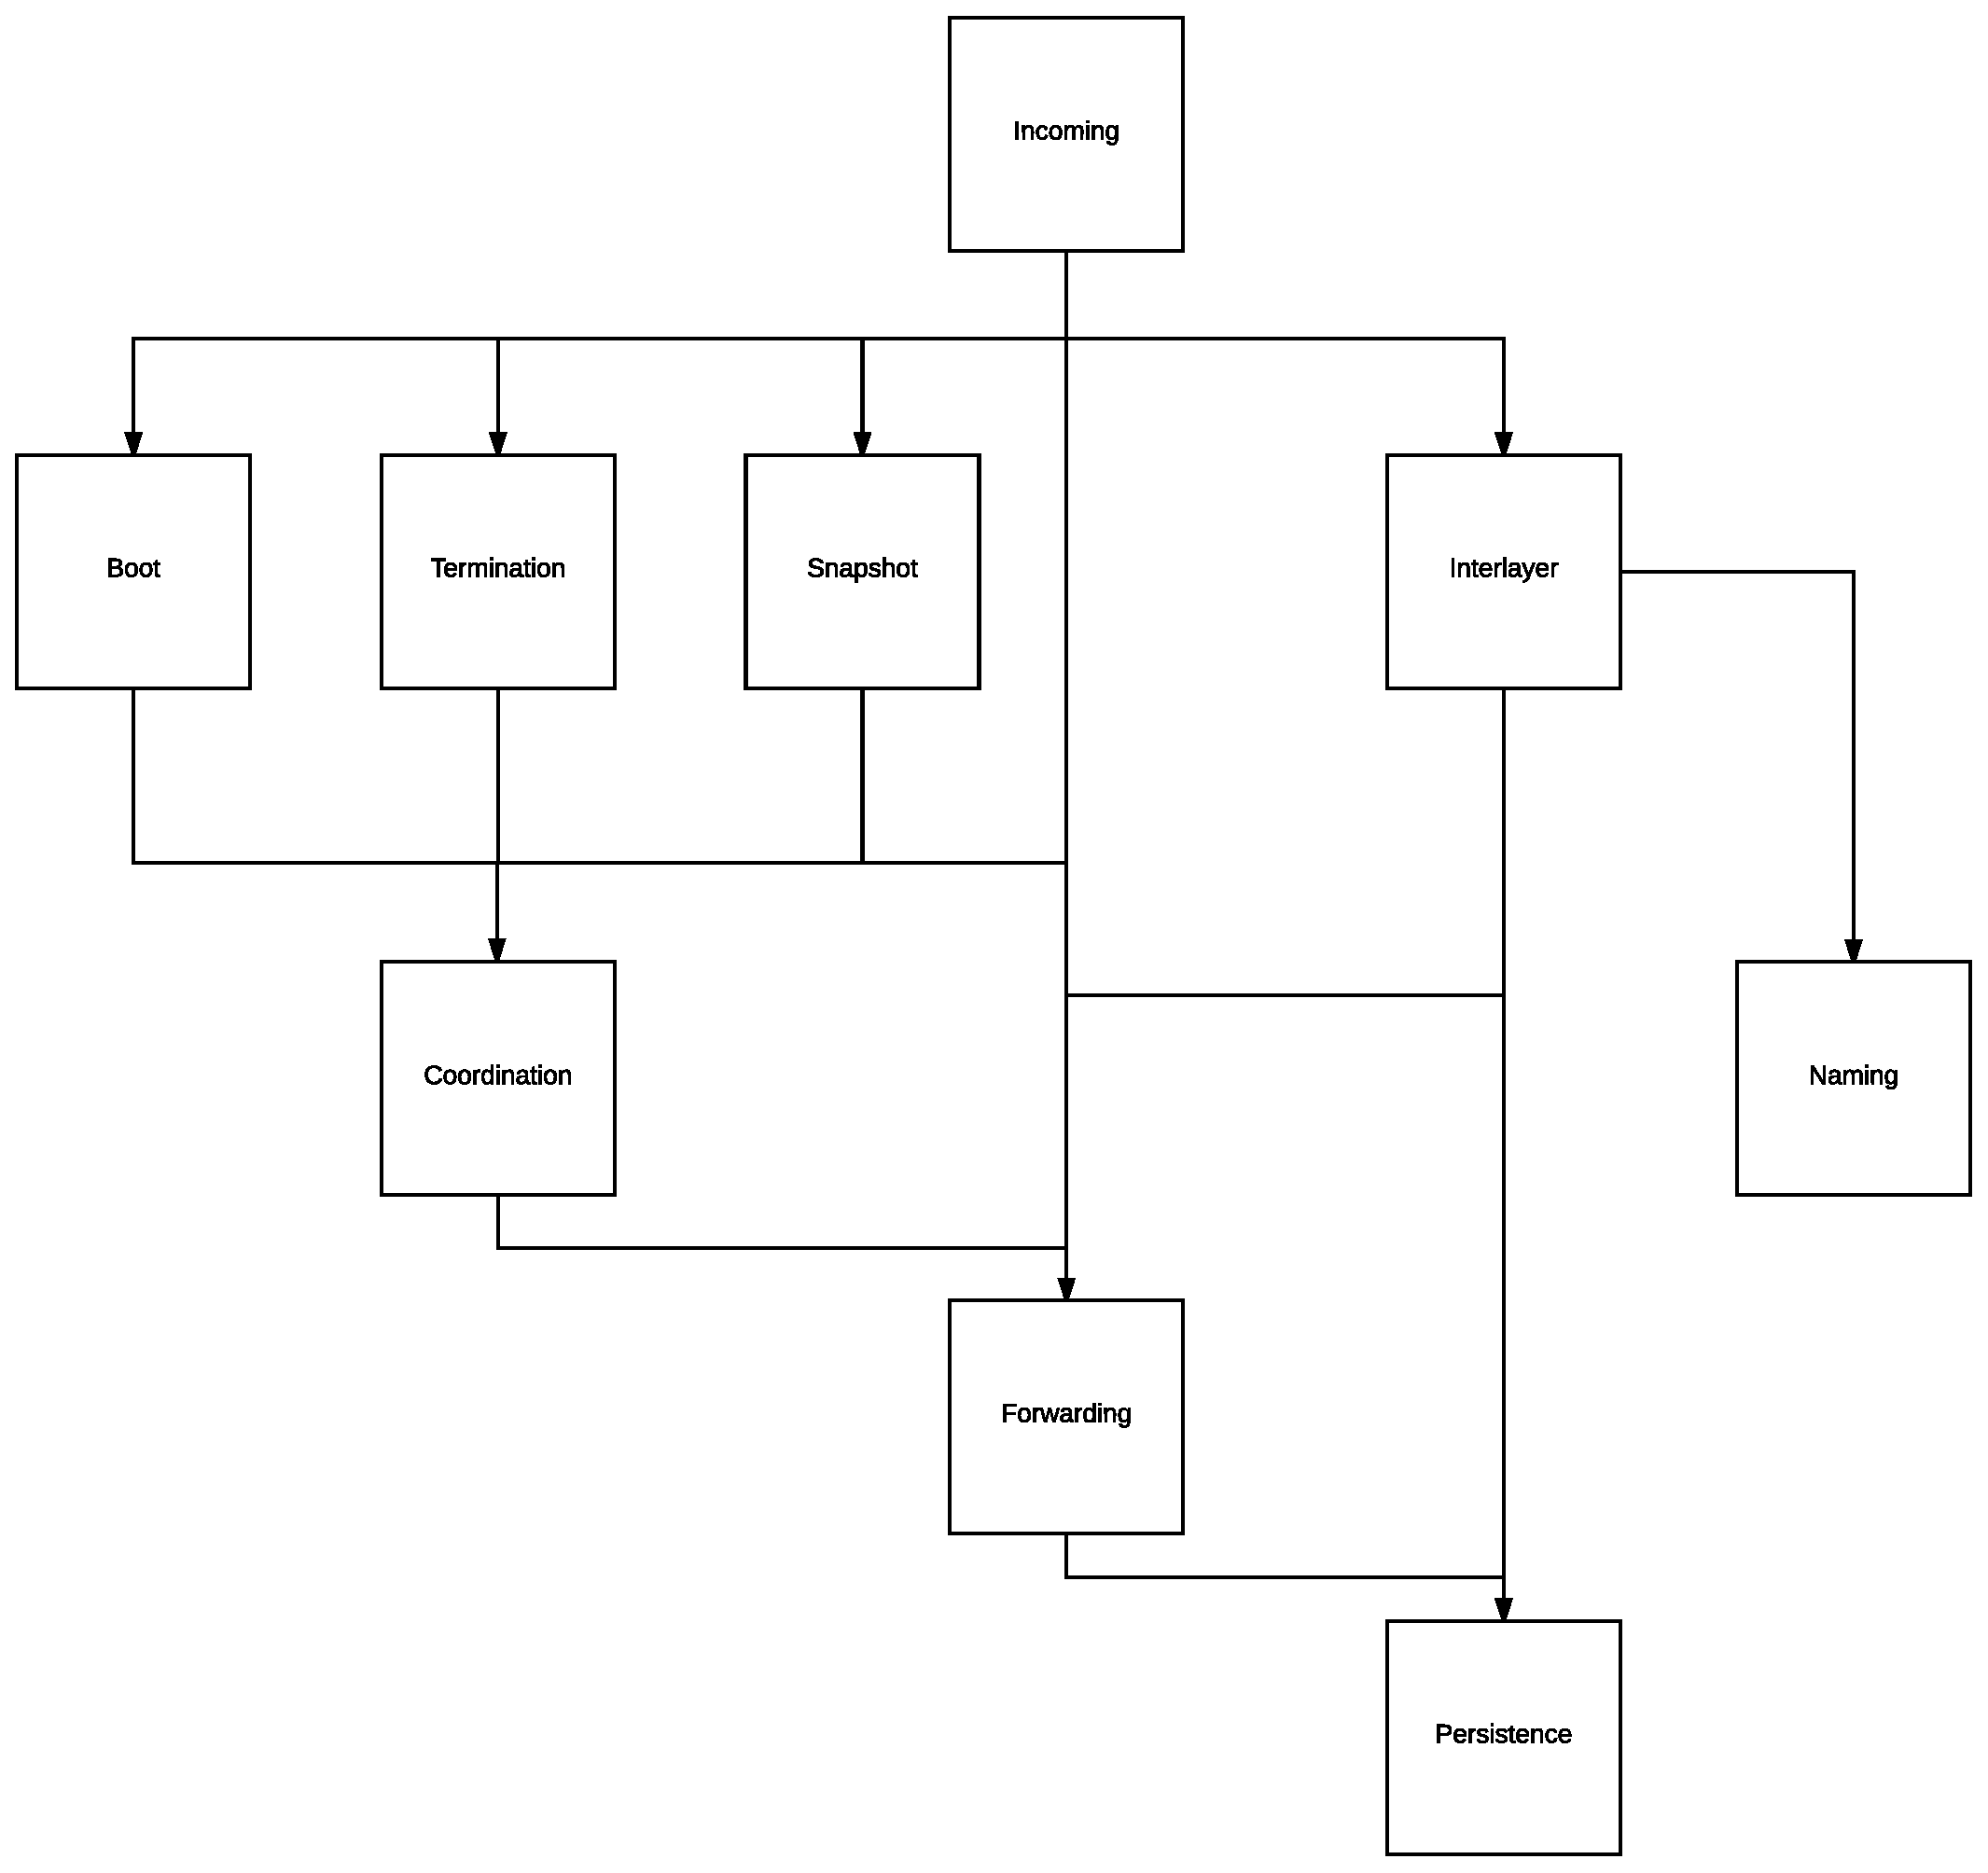
\includegraphics[width=\columnwidth]{images/solution/mw/overview.eps}
  \caption{Middleware architecture overview}
  \label{fig:mw-arch-over}
\end{figure}

\begin{itemize}
  \item \texttt{naming}: service that provides a correspondence between logic
    names and actual network addresses;
  \item \texttt{forwarding}: service that represents the abstraction through
    which it is possible to deliver messages to other middleware nodes;
  \item \texttt{interlayer}: service that represents the interface between
    the application and middleware layers;
  \item \texttt{boot}: service that is responsible to start the system neatly;
  \item \texttt{termination}: service that shut downs the node and the system
    neatly;
  \item \texttt{snapshot}: service that takes consistent views of the node and
    the system;
  \item \texttt{coordination}: service that coordinates the interaction among
    the nodes of the system.
\end{itemize}
